\input preamble.tex
\noindent
\begin{center}
{\bf Oversikt over stasjoner hos 3AUA Gand VGS }
\end{center}
\vskip 5pt
\section{Stasjon 01}

$$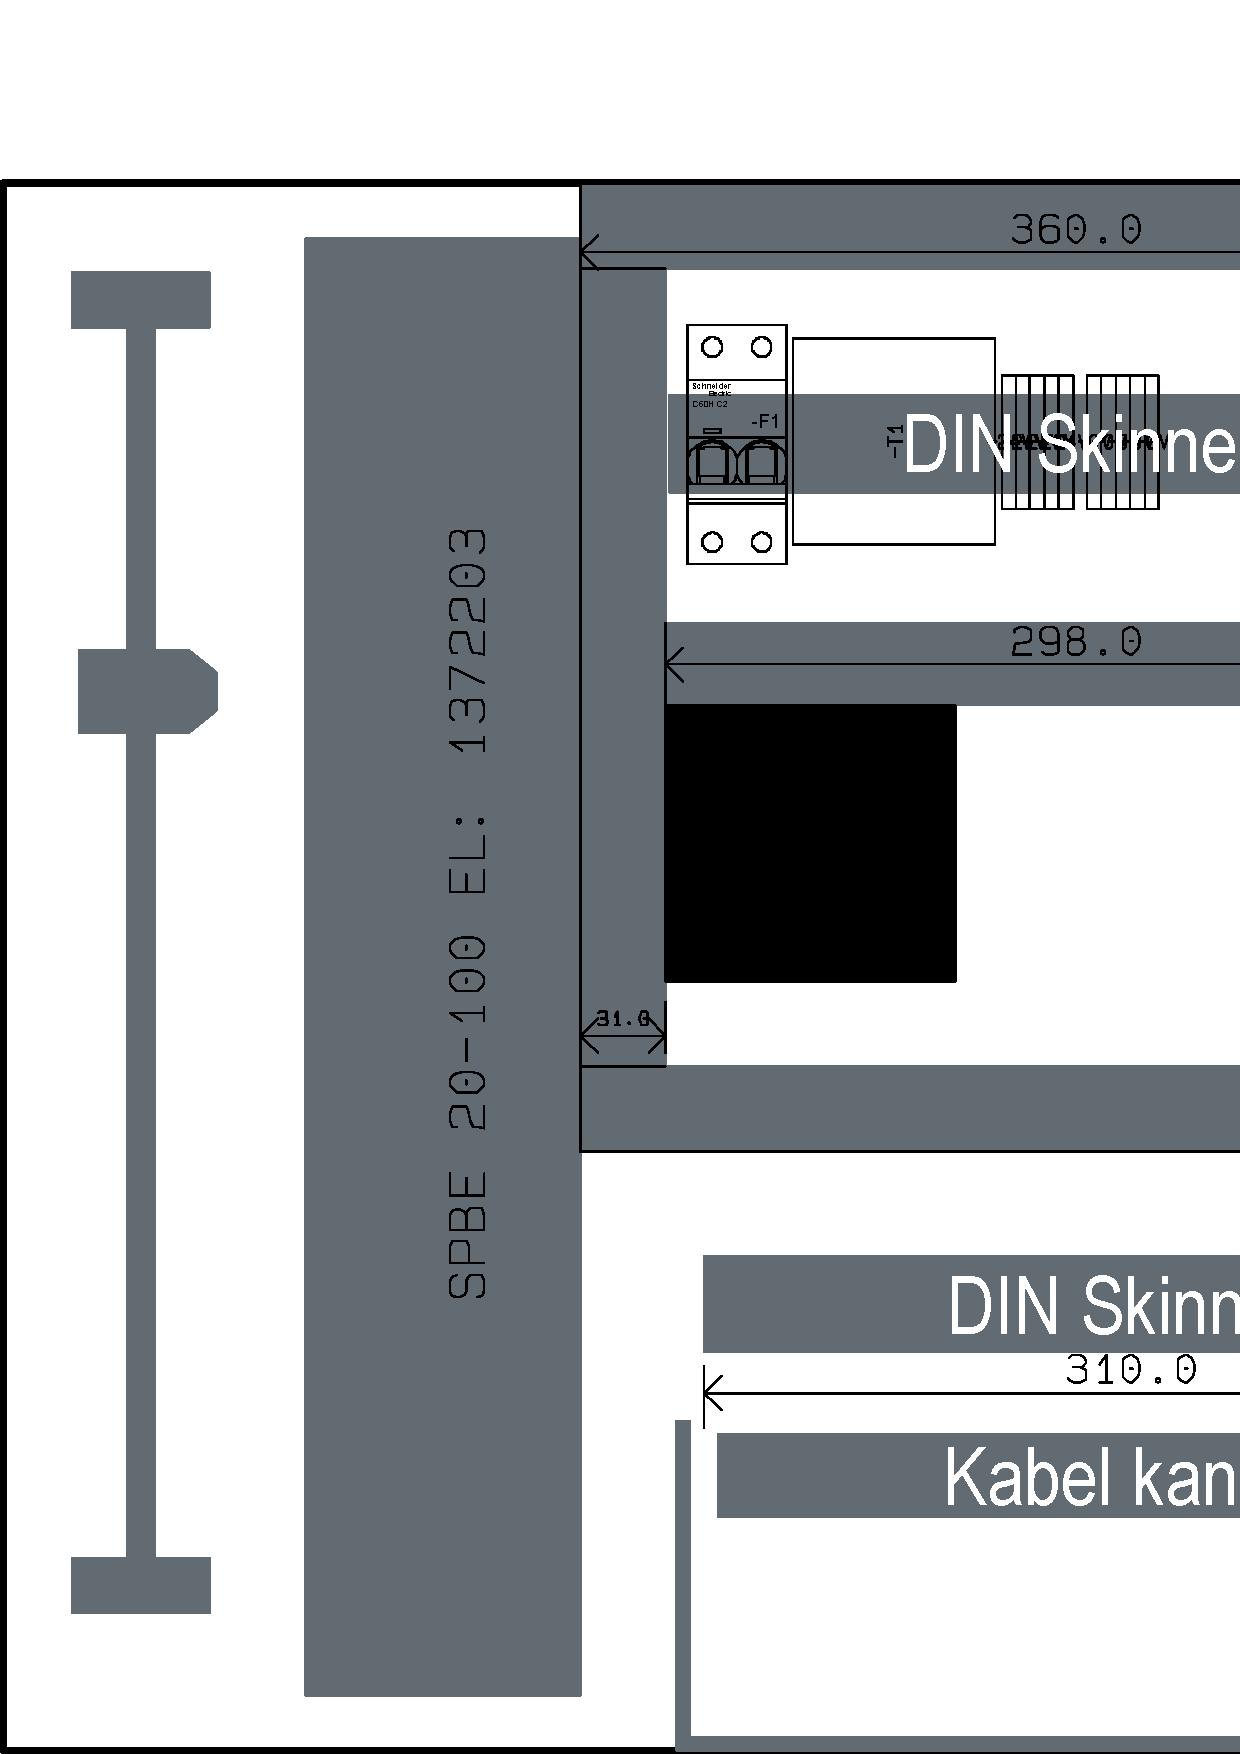
\includegraphics[width=10.5cm,angle=-90]{stasjon01x01.jpg}$$

Stasjon01 - Gandsfjorden Gondol er den første stajsonen vi starter med etter vi er fredige med repitisjon. Det er også den eneste stasjonen der hele klassen jobber med det samme. \\

Hensikten med denne stasjonen er å repitere grunnleggende koblingskunnskap i automasjonsfaget. Her må elevene koble:
\begin{itemize}[noitemsep]
	\item trykkbrytere
	\item ledlamper
	\item treleder nærhetsensorer (kapasitiv og induktiv)
	\item nødstopp og endebrytere som del sikkerhetsrelatert del av styresystemet. 
	\item DC motor med H-bro og PWM styring av hastighet. 
\end{itemize}




Arbeidsoppdraget skal også gjøre elevene kjent med hvordan vi dokumenterer anlegg i 3AUA og bli kjent med PLS programmeringsverktøyet Codesys som vi bruker. 

De skal også montere, konfigurere, kalibre, justere og sette i drift et målesystem for trykk. 

\section{Stasjon 02}

Aktuelle arbeidsoppdrag:

\begin{itemize}[noitemsep]
	\item Sjekk av IO-signaler
	\item dokumentering av nye signaler
	\item Utfordring: fikse analoge signaler
\end{itemize}



$$\includegraphics[width=10.5cm,angle=-90]{stasjon02x01.jpg}$$
Stasjon 02 består av et stort styreskap laget for å styre 5 ulike maskiner, med og uten EXi signaler. Detter er en stasjoner som er under oppbygning. Det er meningen å koble flere og flere stasjoner til  styreskapet. \\




\section{Stasjon 03}

$$\includegraphics[width=10.5cm,angle=-90]{stasjon03x01.jpg}$$

Stasjon 03 er en Gand regueringsstasjon. Den er bygget for å kunne øve på ulike typer regulering. Denne stasjonen brukes til arbeidsoppdrag innen kobling, kalibrering av målesystemer (trykk, nivå strømning), programmering, optimalisering av regulatorer.  På denne stasjonen kan det utføres øvelser med tilbakekoblet regulering (direkte og reverserende), kaskadekoblet regulering og foroverkoblet regulering. 

Aktuelle arbeidsoppdrag:\\

\begin{itemize}[noitemsep]
	\item planlegge, gjennomførte og doumentere oppkobling av stasjonen.
	\item Programmere og lage HMI til stasjonen ut fra gjeldende oppkobling
	\item Optimalisere Z\&N
	\item Optimalisere Skogestad
	\item Optimalisere Kaskadekoblet regulering
	\item Optimalisere Foroverkoblet regulering
	\item Kalibrere DP-celle
	\item Bytte range på dp-celle for nivåmåling
	\item bytte range på ultralyd transmitter
\end{itemize}


\section{Stasjon 04}

$$\includegraphics[width=10.5cm,angle=-90]{stasjon04x01.jpg}$$

Stasjon 04 er en Gand regueringsstasjon. Den er bygget for å kunne øve på ulike typer regulering. Denne stasjonen brukes til arbeidsoppdrag innen kobling, kalibrering av målesystemer (trykk, nivå strømning), programmering, optimalisering av regulatorer.  På denne stasjonen kan det utføres øvelser med tilbakekoblet regulering (direkte og reverserende), kaskadekoblet regulering og foroverkoblet regulering. 

Aktuelle arbeidsoppdrag:\\
\begin{itemize}[noitemsep]
	\item planlegge, gjennomførte og doumentere oppkobling av stasjonen.
	\item Programmere og lage HMI til stasjonen ut fra gjeldende oppkobling
	\item Optimalisere Z\&N
	\item Optimalisere Skogestad
	\item Optimalisere Kaskadekoblet regulering
	\item Optimalisere Foroverkoblet regulering
	\item Kalibrere DP-celle
	\item Bytte range på dp-celle for nivåmåling
	\item bytte range på ultralyd transmitter
\end{itemize}
\section{Stasjon 05}

$$\includegraphics[width=10.5cm,angle=-90]{stasjon05x01.jpg}$$

Stasjon 05 er en reguleringsstasjon gitt til klassen av Kverneland Plogfabrikk. Denne stasjonen er fredig koblet og skal brukes til øvelser i feilsøking. 

Aktuelle arbeidsoppdrag:\\
\begin{itemize}[noitemsep]
	\item Feilsøke ut utbedre feil. 
\end{itemize}


\section{Stasjon 06}

$$\includegraphics[width=10.5cm,angle=-90]{stasjon06x01.jpg}$$

Stasjon 06 er en robot med sikkerhetsbur. Denne brukes til øvelser i robotprogrammering og robot sikkerhet. 


Aktuelle arbeidsoppdrag:\\

\begin{itemize}[noitemsep]
	\item 
\end{itemize}


\section{Stasjon 07}

$$\includegraphics[width=10.5cm,angle=-90]{stasjon07x01.jpg}$$

Stasjon 7 er en brusautomat eller autobar. Denne er under oppbyggning og oppgaver på den vil gå ut på å gjøre den ferdig. 




\section{Stasjon 8}

$$\includegraphics[width=10.5cm,angle=-90]{stasjon08x01.jpg}$$

Stasjon 08 er et XY Aksesystem  for posisjonsregulering med frekvensomformer og servo drive. Denne er også under oppbyggning. 

\section{Stasjon 09}

$$\includegraphics[width=10.5cm]{stasjon09x01.jpg}$$

Stasjon 09 eller de tre tanker er en litt større reguleringsstasjon der vannet pumpes fra  et resovoar og gjennom tre tanker før det sleppes tilbake til resovoaret. Her kan en gjøre øvelser med HMI bygging, innstilling av regulatorene og øvelser på ulike nivåmålesystem. 

Aktuelle arbeidsoppdrag:\\
\begin{itemize}[noitemsep]
	\item planlegge, gjennomførte og doumentere oppkobling av stasjonen.
	\item Programmere og lage HMI til stasjonen ut fra gjeldende oppkobling
	\item Optimalisere Z\&N
	\item Optimalisere Skogestad
	\item Sette i stand målesystem med DP-celle i tett tank for måling av nivå
	\item Bytte range på dp-celle for nivåmåling
	\item bytte range på ultralyd transmitter
\end{itemize}


\section{Stasjon 10}

$$\includegraphics[width=10.5cm,angle=-90]{stasjon10x01.jpg}$$

Stasjon 10 er for benkkalibrering av trykksensorer. 
Aktuelle arbeidsoppdrag:\\
\begin{itemize}[noitemsep]
	\item kalibrering av ulike trykksensorer
	\item Læringsoppdrag for målesystemer med trykk
\end{itemize}
\section{Stasjon 11}

$$\includegraphics[width=10.5cm,angle=-90]{stasjon11x01.jpg}$$

Stasjon 11 er for benkkalibrering av temperatursensorer. 
Aktuelle arbeidsoppdrag:\\
\begin{itemize}[noitemsep]
	\item kalibrering av temperatursensorer og temperaturtransmittere
	\item Læringsoppdrag for målesystemer med temperatur
\end{itemize}

\section{Stasjon 12}

$$\includegraphics[width=10.5cm]{stasjon12x01.jpg}$$

Stasjon 12 er et ventilasjonsaregat der instrumenteringen er gitt til oss av KE Automasjon. Denne stasjonen brukes til øvelser på sensorer og pådragsorganer som normalt byrukes i byggautomasjon og programmeringsøvelser på ukjent PLS. På stasjonen står det en B\&R PLS, denne følger standarden EN 61131-3 for prgrammering av pls. Det vil si at den har mange likeheter med programmering i Codesys. 

Aktuelle arbeidsoppdrag:\\
\begin{itemize}[noitemsep]
	\item IO-sjekk av signaler
	\item programmering av ventilasjonsaregat
\end{itemize}
\section{Stasjon 13}

$$\includegraphics[width=10.5cm]{stasjon13x01.jpg}$$

Aktuelle arbeidsoppdrag:\\
\begin{itemize}[noitemsep]
	\item 
\end{itemize}

\section{Stasjon 14}

$$\includegraphics[width=10.5cm,angle=-90]{stasjon14x01.jpg}$$

Aktuelle arbeidsoppdrag:\\
\begin{itemize}[noitemsep]
	\item 
\end{itemize}

\section{Stasjon 15}

$$\includegraphics[width=10.5cm]{stasjon15x01.jpg}$$

Aktuelle arbeidsoppdrag:\\
\begin{itemize}[noitemsep]
	\item 
\end{itemize}

\section{Stasjon 16}

$$\includegraphics[width=10.5cm]{stasjon16x01.jpg}$$

Aktuelle arbeidsoppdrag:\\
\begin{itemize}[noitemsep]
	\item 
\end{itemize}

\section{Stasjon 17}

$$\includegraphics[width=10.5cm]{stasjon17x01.jpg}$$

Aktuelle arbeidsoppdrag:\\
\begin{itemize}[noitemsep]
	\item 
\end{itemize}

\section{Stasjon 18}

$$\includegraphics[width=10.5cm]{stasjon18x01.jpg}$$

Aktuelle arbeidsoppdrag:\\
\begin{itemize}[noitemsep]
	\item 
\end{itemize}

\section{Stasjon 19}

$$\includegraphics[width=10.5cm]{stasjon19x01.jpg}$$

Aktuelle arbeidsoppdrag:\\
\begin{itemize}[noitemsep]
	\item 
\end{itemize}


\section{Stasjon 20}

$$\includegraphics[width=10.5cm]{stasjon20x01.jpg}$$

Aktuelle arbeidsoppdrag:\\
\begin{itemize}[noitemsep]
	\item 
\end{itemize}








































\end{document}


